\PassOptionsToPackage{table}{xcolor}
\documentclass[aspectratio=169,xcolor=dvipsnames,11pt]{beamer}
\usetheme{SimplePlusAIC}
\usepackage{amsmath}
\usepackage{animate}
\usepackage{hyperref}
\usepackage{cleveref}
\usepackage{caption}
\usepackage{graphicx} % Allows including images
%\usepackage{subfig}
\usepackage{subcaption}
\usepackage{booktabs} % Allows the use of \toprule, \midrule and  \bottomrule in tables
\usepackage{svg} %allows using svg figures
\usepackage{tikz}
\usetikzlibrary{intersections}
\usetikzlibrary{arrows.meta, calc, quotes, tikzmark}
\usepackage{makecell}
\usepackage{multirow}
\usepackage{appendixnumberbeamer}
\usepackage{wrapfig}
\usepackage{verbatim}
\usepackage{tcolorbox}
%\usepackage[dvipsnames]{xcolor}

\usepackage{hhline}
\usepackage{relsize}
\usepackage{bm}
%Select the Epilogue font (requires luaLatex or XeLaTex compilers)
%\setsansfont{Epilogue}[
  %  Path=./epilogueFont/,
  %  Scale=0.9,
  %  Extension = .ttf,
   % UprightFont=*-Regular,
   % BoldFont=*-Bold,
   % ItalicFont=*-Italic,
    %BoldItalicFont=*-BoldItalic
    %]
    \usefonttheme[onlymath]{serif}
% \usepackage{ eulervm } % Euler VM as math serif font

\newcommand*{\defeq}{\stackrel{\text{def}}{=}}
\newcommand{\grad}{\nabla}
\newcommand{\lap}{\Delta}
\newcommand{\weaklyto}{\rightharpoonup}
\newcommand{\weakstar}{\stackrel{*}\rightharpoonup}
\newcommand{\cts}{\hookrightarrow}
\newcommand{\ctsDense}{\xhookrightarrow{d}}
\newcommand{\ctsCompact}{\xhookrightarrow{c}}
\newcommand{\E}{\mathbb{E}}
\newcommand{\pP}{\mathbb{P}}
\newcommand{\R}{\mathbb{R}}
\newcommand{\ER}{\overline{\mathbb{R}}}
\newcommand{\cR}{\mathcal{R}}
\newcommand{\cJ}{\mathcal{J}}
\newcommand{\cG}{\mathcal{G}}
\newcommand{\CVaR}{\textup{CVaR}}
\newcommand{\D}{\textup{ d}}
\newcommand{\dd}{\mathrm{d}}
\newcommand{\fa}{\text{for all }}
\DeclareMathOperator*{\essinf}{\vphantom{p}ess\,inf}
\DeclareMathOperator{\sigmoid}{expit} % a.k.a. logistic sigmoid

\usepackage[ruled,vlined,algo2e]{algorithm2e}
\crefname{algocf}{algorithm}{algorithms}
 \usepackage{caption}

\usepackage{tcolorbox}  % For fancy boxes
\usepackage{lipsum}     % For dummy text

% Define a custom style for the box
\tcbuselibrary{skins, breakable}
\newtcolorbox[auto counter, number within=section]{roundedshadowbox}[2][]{
    colback=white, % Background color (kept white)
    colframe=black, % Border color
    boxrule=0.5pt, % Border thickness
    arc=5mm, % Rounded corners
    shadow=true, % Drop shadow effect
    width=\linewidth, % Full width box
    title=#2, % Title text
    #1 % Additional options (e.g., width override)
}

\usepackage{pgfplots}
\pgfplotsset{compat=1.18}

%\PassOptionsToPackage{table}{xcolor}
%\documentclass[aspectratio=169,xcolor=dvipsnames,11pt]{beamer}
%\usetheme{SimplePlusAIC}
%\usepackage{amsmath}
%\usepackage{hyperref}
%\usepackage{cleveref}
%\usepackage{caption}
%\usepackage{graphicx} % Allows including images
%\usepackage{subcaption}
%\usepackage{booktabs} % Allows the use of \toprule, \midrule and  \bottomrule in tables
%\usepackage{svg} %allows using svg figures
%\usepackage{tikz}
%
%\usepackage{pgfplots}
%\pgfplotsset{compat=1.18}
%
%\usepackage{makecell}
%\usepackage{multirow}
%\usepackage{appendixnumberbeamer}
%\usepackage{wrapfig}
%\usepackage{verbatim}
%\usepackage{tcolorbox}
%\usepackage{hhline}
%\usepackage{relsize}
%\usepackage{bm}
%
%\usefonttheme[onlymath]{serif}
%    
\newcommand{\C}{\mathbb C}

%
%%\font\nullfont=cmr10
%
%\usepackage{tcolorbox}  % For fancy boxes
%\usepackage{lipsum}     % For dummy text
%
%% Define a custom style for the box
%\tcbuselibrary{skins, breakable}
%\newtcolorbox[auto counter, number within=section]{roundedshadowbox}[2][]{
%    colback=white, % Background color (kept white)
%    colframe=black, % Border color
%    boxrule=0.5pt, % Border thickness
%    arc=5mm, % Rounded corners
%    shadow=true, % Drop shadow effect
%    width=\linewidth, % Full width box
%    title=#2, % Title text
%    #1 % Additional options (e.g., width override)
%}


%----------------------------------------------------------------------------------------
%	TITLE PAGE
%----------------------------------------------------------------------------------------

\title[\quad\quad\quad LVPP Course III]{The Latent Variable Proximal Point Method III: LVPP for Free Discontinuity Problems, Nonlinear PDEs and Future Directions
 } % The short title appears at the bottom of every slide, the full title is only on the title page
%\subtitle{Subtitle}

\author{\small{\bf Thomas M. Surowiec}}

\institute[T.M. Surowiec]{Department of Numerical Analysis and Scientific Computing \newline Simula Research Laboratory \newline Oslo, Norway}
% Your institution as it will appear on the bottom of every slide, maybe shorthand to save space


\date[EMS School]{ {\footnotesize 
K\'acov, Czechia, 15-20 June 2025}}
%----------------------------------------------------------------------------------------
%	PRESENTATION SLIDES
%----------------------------------------------------------------------------------------

\begin{document}

{
\setbeamertemplate{background canvas}{}
\frame{\titlepage}
}

\begin{frame}{Overview}
\tableofcontents
\end{frame}


\section{Legendre Functions and Geometry Preserving Transformations}
\begin{frame}\frametitle{The LVPP Team}
\captionsetup[subfigure]{labelformat=empty}
\begin{figure}
  \begin{subfigure}[b]{2.75cm}
    \includegraphics[width=\linewidth,height=2.5cm, keepaspectratio]{figures/bren096.jpg}
    \caption{Brendan Keith\\ Brown University}
  \end{subfigure}
  \hfill
  \begin{subfigure}[b]{2.75cm}
    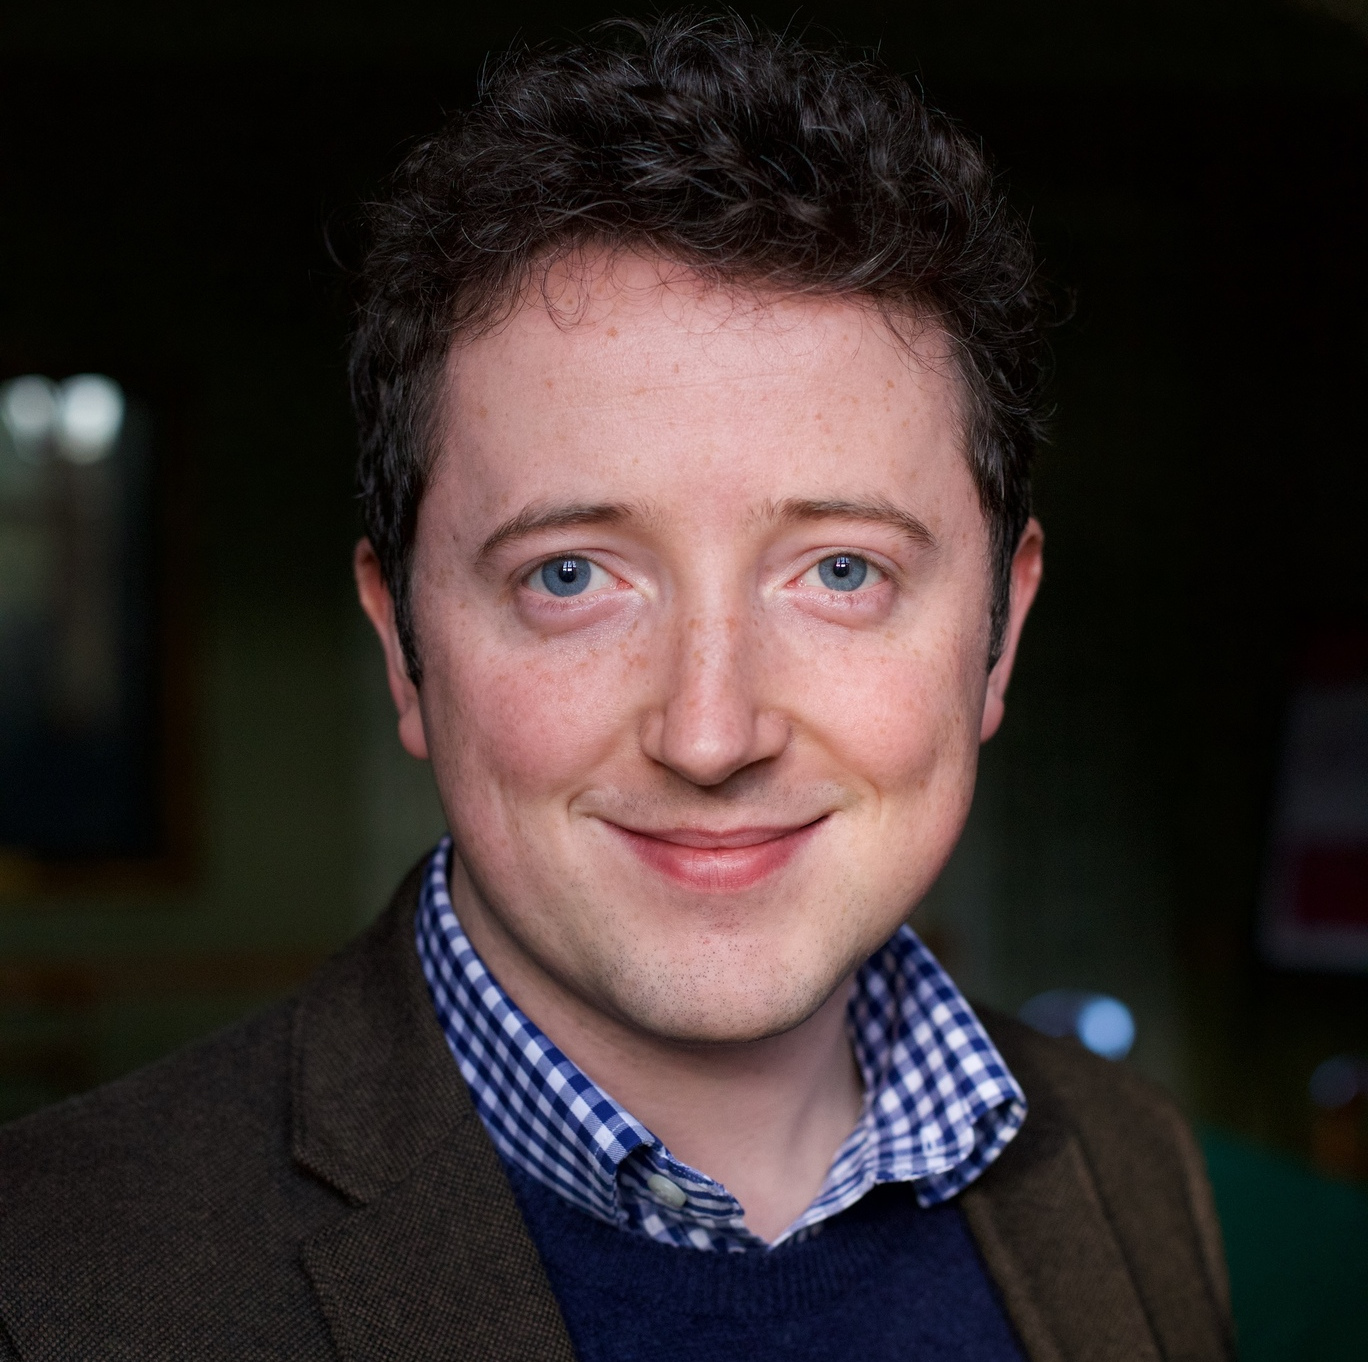
\includegraphics[width=\linewidth,height=2.5cm, keepaspectratio]{figures/patrick.jpg}
    \caption{Patrick E. Farrell\\ Oxford University}
  \end{subfigure}
  \hfill
  \begin{subfigure}[b]{2.75cm}
    
\includegraphics[width=\linewidth,height=2.5cm, keepaspectratio]{figures/joergen.png}
    \caption{Jorgen S. Dokken\\ Simula Research Lab}
  \end{subfigure}
   \hfill
  \begin{subfigure}[b]{3.2cm}
    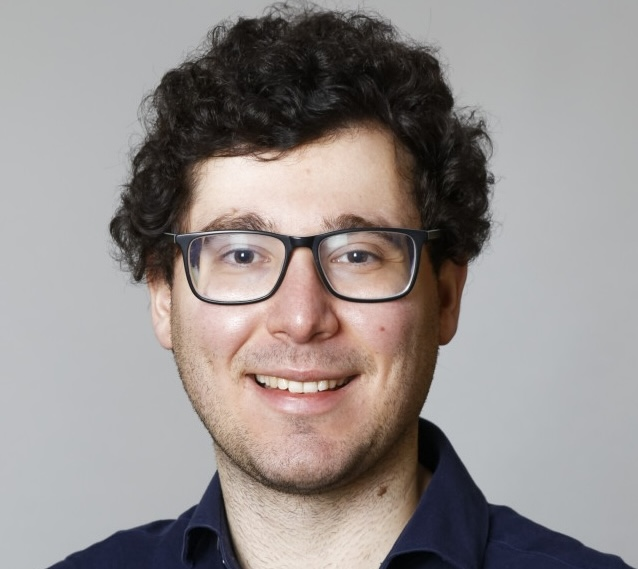
\includegraphics[width=\linewidth,height=2.5cm, keepaspectratio]{figures/papadopoulos.jpg}
    \caption{Ioannis Papadopoulos\\ Weierstra\ss-Institut}
  \end{subfigure}
\hspace{7em}	
%  \hfill
%  \begin{subfigure}[b]{0.19\textwidth}
%    \includegraphics[width=\linewidth]{figures/rivers.jpg}
%    \caption{Diffusive Waves}
%  \end{subfigure}
\end{figure}\vspace{-4ex}
{\tiny
\begin{thebibliography}{1}

\bibitem{BKeith_TMSurowiec_2024}
{\sc B.~Keith and T.M.~Surowiec.}
\newblock Proximal Galerkin: A structure‐preserving finite element method for pointwise bound constraints
\newblock Found. Comut. Math. (2024), \url{https://doi.org/10.1007/s10208-024-09681-8}

\bibitem{JSDokken_etal_2025}
{\sc J.S.~ Dokken, P.E.~Farrell, B.~Keith, I.P.A.~Papadopolous and T.M.~Surowiec.}
\newblock The latent variable proximal point algorithm for variational problems with inequality constraints
\newblock In review (after minor revision) (2025), \url{https://arxiv.org/abs/2503.05672}
\end{thebibliography}
}
\end{frame}

  \begin{frame}\frametitle{Quadratic Penalty Methods}
  \begin{minipage}{0.67\linewidth}
\begin{beamercolorbox}[rounded=true, shadow=true, wd=\textwidth]{block body}
 Given $\gamma > 0$, we seek a minimizer $u_{\gamma} \in H^1_0(\Omega)$ of the objective functional:
 \begin{equation*}
 	J_{\gamma}(v)
 	=
 	\frac{1}{2}
 	\int_\Omega |\nabla v|^2 \dd x
 	-
 	\int_\Omega f v\dd x
	+
	\underbrace{\frac{\gamma}{2}\int_{\Omega} \max\{0,\varphi - v\}^2 \dd x}_{=:\gamma \beta(v)}
 	\,.
 \end{equation*}
 Here, $f \in L^2(\Omega)$ and  $\varphi \in H^1(\Omega)$, $\varphi|_{\Gamma} \le 0$.
\end{beamercolorbox}
\end{minipage}\hfill
\begin{minipage}{0.3\linewidth}
 \begin{figure}
% \resizebox{0.3\textwidth}{0.25\textwidth}{%
  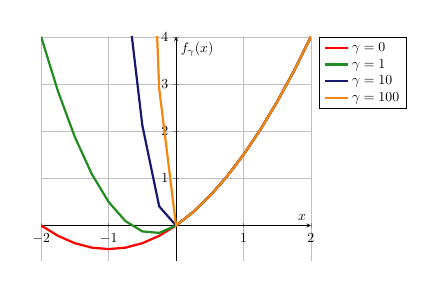
\begin{tikzpicture}[scale=0.5]
    \begin{axis}[
        axis lines=middle, % Draw axes through the origin
        xlabel=$x$,
        ylabel=$f_\gamma(x)$,
        xmin=-2, xmax=2, % Adjust x-range as needed
        ymin=-0.75, ymax=4, % Adjust y-range as needed
        grid=both, % Add a grid
        grid style={line width=.1pt, draw=gray!10}, % Style the grid lines
        major grid style={line width=.2pt,draw=gray!50}, % Style major grid lines
        xtick distance=1, % Tick marks every 1 unit on x-axis
        ytick distance=1, % Tick marks every 1 unit on y-axis
        % Add a legend
        legend pos=outer north east, % Position the legend
        legend cell align=left,
        no markers, % Don't put markers on the plots
    ]

    % Define the function with a placeholder for c
    % We use 'max(0,x)^2' for the (x)^2 part, and then multiply by c
    % PGFPlots works with degrees, so we need to be careful with functions that are not trigonometric.
    % max(0, x) is directly supported.


    \addplot[domain=-2:4, Red, ultra thick] {0.5*x^2 + 1*x + 0 * max(0,-x)^2};
    \addlegendentry{$\gamma=0$};
    % Plot for c = 0.5
    \addplot[domain=-2:4, ForestGreen, ultra thick] {0.5*x^2 + 1*x + 1 * max(0,-x)^2};
    \addlegendentry{$\gamma=1$};

    % Plot for c = 1
    \addplot[domain=-2:4, MidnightBlue, ultra thick] {0.5*x^2 + 1*x + 10.0 * max(0,-x)^2};
    \addlegendentry{$\gamma=10$};

    % Plot for c = 2
    \addplot[domain=-2:4, BurntOrange, ultra thick] {0.5*x^2 + 1*x + 50.0 * max(0,-x)^2};
    \addlegendentry{$\gamma=100$};

    \end{axis}
\end{tikzpicture}
%}
\caption{\scriptsize Plot of $f_\gamma(x) = \frac{1}{2} x^2 + x + \gamma\max\{0,-x\}^2$}
  \label{fig:tikz-example}
\end{figure}
\end{minipage}
  \end{frame}

\begin{frame}\frametitle{A}
\begin{itemize}
\item Recall what we did with Bregman proximal point and use the graphic from the Austin talk
\item The key to developing an abstract LVPP framework for more general constraints lies in the way we construct the Bregman divergence.
\item As you may recall, the Bregman divergence gives us the linearization error of a particular type of proper, convex, lower-semicontinuous function $R$
\item The Bregman divergence is not symmetric, but it is always non-negative on its domain.
\item We will now take a deeper look at an important class of convex functions called \alert{Legendre functions}
\end{itemize}
\end{frame}

\begin{frame}\frametitle{A}
\begin{itemize}
\item Define proper, convex, lsc again
\item Define convex conjugate and motivate its meaning
\item Define Legendre function
\item Find a picture of Rockafellar
\item Work out two examples to show how to compute the convex conjugate
\item Prove (if possible) the crucial Rockafellar theorems
\item Give the table in the paper
\item Return to Bregman 
\end{itemize}
\end{frame}

\begin{frame}\frametitle{A}
\begin{itemize}
\item
\end{itemize}
\end{frame}

\begin{frame}\frametitle{A}
\begin{itemize}
\item
\end{itemize}
\end{frame}

\begin{frame}\frametitle{A}
\begin{itemize}
\item
\end{itemize}
\end{frame}

\begin{frame}\frametitle{A}
\begin{itemize}
\item
\end{itemize}
\end{frame}

\begin{frame}\frametitle{A}
\begin{itemize}
\item
\end{itemize}
\end{frame}

\section{The General LVPP Algorithm}
\begin{frame}\frametitle{A}
\begin{itemize}
\item
\end{itemize}
\end{frame}

\section{Applications}
\begin{frame}\frametitle{A}
\begin{itemize}
\item
\end{itemize}
\end{frame}

\end{document}